\subsection{Sicherheitskritische Aspekte der SOA}
\label{sec:securityAspects}

Eine serviceorientierte Architektur ist ohne IT-Sicherheit nicht denkbar. Neben klassischen, bei jeder IT-Lösung, auftretenden Aufgaben gibt es auch - durch den verteilten Ansatz von SOA - spezielle Anforderungen an das System \cite{BITKOM.2009}.

Die einzelnen Aufgaben müssen dabei nicht neu erfunden werden, sondern haben lediglich besondere Ausprägungen in der Anwendung von SOA. In allen Fällen muss sich mit folgenden Problemen befasst werden \cite{BITKOM.2009}:\begin{itemize}
    \item Identitätsverwaltung
    \item Authentisierung
    \item Autorisierung (=Access Control)
    \item und die verschlüsselte Kommunikation zwischen den Diensten.
\end{itemize}

Nachfolgend wird beschrieben, wieso diese Aufgaben gerade in SOA kritische Herausforderungen sind und wie sie gelöst werden.

\paragraph{Access Control:}

In einer SOA müssen nicht nur viele Benutzer, sondern auch Dienste authentifiziert werden. Die Verwaltung dieser Identitäten, insbesondere über Organisationsgrenzen hinweg ist eine Notwendigkeit \cite{BITKOM.2009}.

Bei SOA existieren - anders als bei monolithischen Architekturen - viele potenzielle Schwachstellen an jedem Service. Wird eine davon ausgenutzt, so ist zwar nur ein kleiner Teil der Anwendung kompromittiert, aber die Sicherheit des Gesamten ist nicht mehr vorhanden.

Jeder einzelne Service sollte ausreichend mit geschützt sein, damit nur autorisierte Identitäten Zugriff auf eine Ressource haben. Gleichzeitig sollten Benutzer sich nicht bei jedem Service einzeln anmelden, da es nicht benutzerfreundlich ist.

Dies kann erreicht werden, indem bestehende Sicherheits-Architekturen oder Standards in SOA als weitere Services integriert werden. Der Hauptzweck hinter all diesen Standards ist die Orchestrierung der Authentifizierung zwischen mehreren Diensten.

Die dabei am häufigsten verwendeten Standards sind:\begin{itemize}
    \item \textbf{XACML}: Dieser Standard besteht aus mehreren Services (Points), welche anhand von Policies Anfragen einer Entität bewerten und gegebenenfalls weiterleiten. \glqq XACML bleibt die einzige standardisierte Methode zur dynamischen Durchsetzung von Autorisierungen, indem Zugriffskontrollen von Anwendungen und Datenbanken ausgelagert und Geschäftsrichtlinien verwendet werden.\grqq{} \cite{Axiomatics.03.08.2022}\\
    \begin{figure}[H]
        \centering
        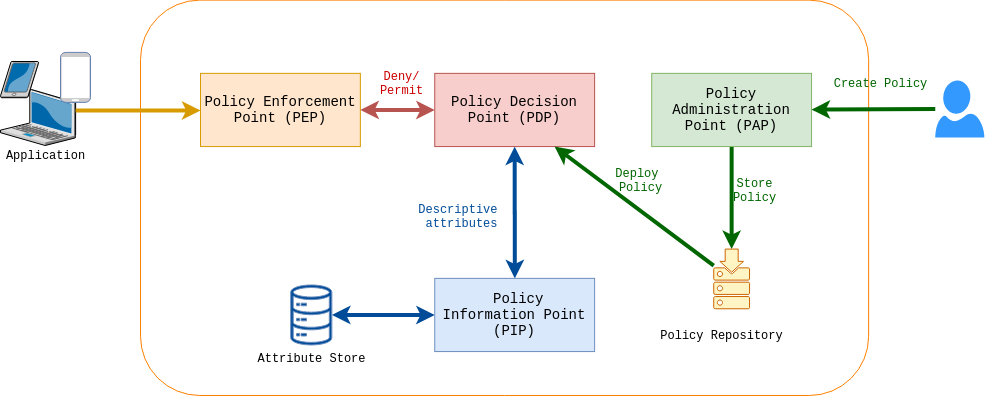
\includegraphics[width=.8\textwidth]{images/XACML.png}
        \caption{XACML Flow-Diagramm}
    
    \end{figure}
    \item \textbf{SAML2}: Hierbei exisitiert ein Identity Provider, an den jeder Service \glqq weiterleitet\grqq{}, um zentral an einer Stelle die Autorisierung zu überprüfen. \cite{Wisniewski.2006}\\
    \begin{figure}[H]
        \centering
        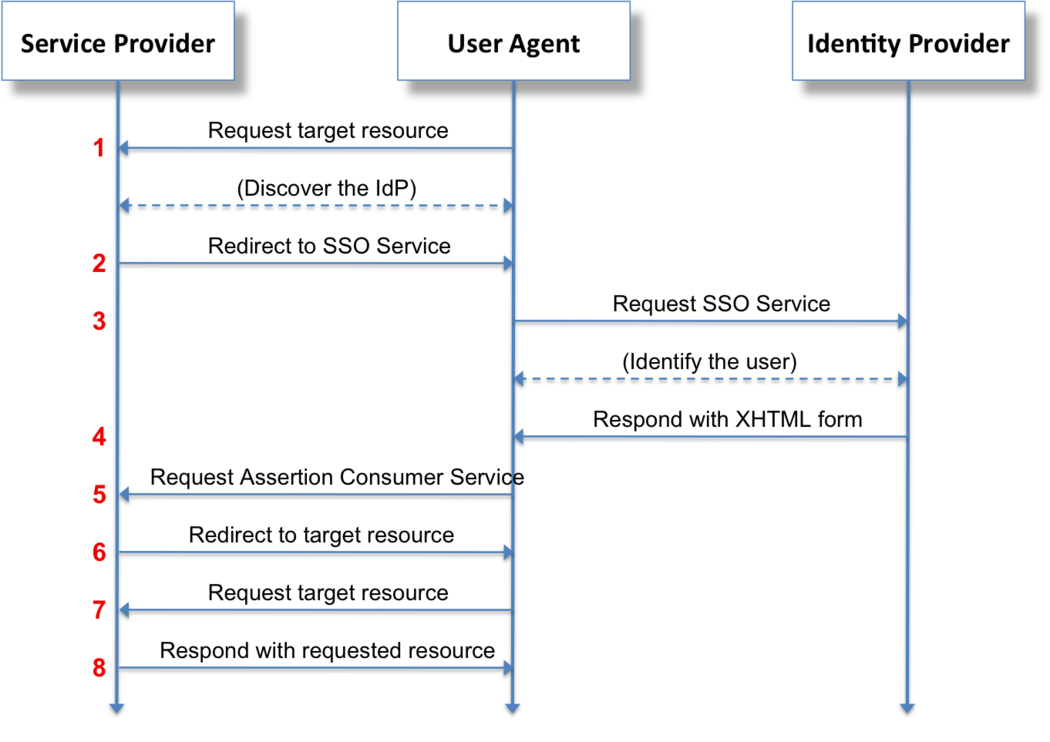
\includegraphics[width=.6\textwidth]{images/SAML.png}
        \caption{SAML Sequenz-Diagramm}
    
    \end{figure}
\end{itemize}

Die detaillierte Beschreibung dieser Standards würde den Rahmen dieser Arbeit übersteigen. Es existieren jedoch viele Ressourcen, um sich diese näher anzusehen.

\paragraph{Verschlüsselung:}
Neben den Diensten selbst, stellen auch die Kommunikationskanäle dazwischen einen Angriffsvektor dar, da diese meist Netzwerkprotokolle verwenden. Um die Integrität, Vertraulichkeit und die Authentizität der Nachrichten zu erfüllen wird der WS-Security (Web-Service Security) Standard verwendet.

WS-Security baut auf SOAP auf und klärt:\begin{itemize}
    \item Wie SOAP-Nachrichten signiert werden um die Integrität sicherzustellen.
    \item Wie SOAP-Nachrichten verschlüsselt werden um Vertraulichkeit zu gewährleisten.
    \item Wie Sicherheitstokens an SOAP-Nachrichten angehängt werden können um die Identität des Absenders sicherzustellen.
\end{itemize}

Die WSS-Spezifikation gibt nicht explizit vor, welche Signaturformate, Verschlüsselungsalgorithmen oder Sicherheits-Token Modelle verwendet werden müssen. Somit kann dieser für die Zukunft geändert werden, falls bessere und neuere Modelle existieren.

Das große Problem bei der Kanalverschlüsselung in SOA ist die große Anzahl der Kanäle. Egal welche Sicherheitsmaßnahmen eingesetzt werden, sie werden immer die Performance beeinträchtigen. 

WSS ist ca. 8 Mal langsamer als herkömmliches HTTPS \cite{Lascelles.2006}, bietet jedoch sichere Funktionalitäten. 

Ein großer Performanceverlust liegt in der Generierung eines neuen Schlüssels für jede geschickte Nachricht. Als Upgrade existiert WSS-Conversation (WSSC), welches gleichzeitige Sessions unterstützt, ohne einen Schlüssel neu definieren zu müssen (verdoppelt den durchschnittlichen Durchsatz) \cite{Lascelles.2006}. 